%%%%%%%%%%%%%%%%%%%%%%%%%%%%%%%%%%%%%%%%%%%%%%%%%%%%%%%%%%%%%%%%%%%%%%%%%%%%%%%%
%						METHOD												   %
%%%%%%%%%%%%%%%%%%%%%%%%%%%%%%%%%%%%%%%%%%%%%%%%%%%%%%%%%%%%%%%%%%%%%%%%%%%%%%%%
\subsection{Target Device}
The evaluation has been conducted on the polymorphism dataset presented in \autoref{sec:claps_ds}.
We remarked then that the \glspl{snr} computed on both \mbedTLS{} and \aeshuitbit{} implementations protected with code polymorphism did not reveal any leakage, although a re-alignment process was suggested to annihilate the misalignment effect of the counter-measure -- see \autoref{sec:claps_ds}.
In \autoref{sec:realignment_claps}, we propose a way to re-align the traces on the \mbedTLS{} dataset.


\subsection{Threat Models}
\label{sec:threat_models}
We propose several threat models that we distinguish according to two resources the attacker may access, that we precise hereafter.

First, the attacker may get or not an open sample in order to conduct a profiled attack scenario, as considered in this thesis.
We recall that this is a necessary condition in order to evaluate the worst-case scenario from a developer's point of view~\cite{heuser_good_2014}.
Though often seen as strong, this assumption can be considered as realistic in our context: here both the chip and the source codes used for the evaluation are publicly available.

Second, the attacker may eventually incorporate human expertise to improve attacks initially fully automatized.
Here, this will concern either the preliminary task of trace re-alignment (see the procedure described in \autoref{sec:realignment_claps}), or the capacity to  properly design a CNN architecture for the deep learning based \gls{sca} (see \autoref{sec:cnn_archi_esorics}).

Hence the following attack scenarios:
\begin{itemize}
	\item \textbf{\attLDADesync{}:} considers a fully automatized attack (\ie{} without any human expertise), without access to any open sample.
	\item \textbf{\attCPASync{}:} considers an attack without access to an open sample, but with human expertise to re-align the traces -- see \autoref{sec:realignment_claps}.
	It results in doing a \gls{cpa} targeting the output of the \sub{} operation, assuming the Hamming weight leakage model -- see \autoref{sec:non_profiled_attacks}.
	\item \textbf{\attLDASync{}:} considers the same attack as \attCPASync{}, \ie{} targeting re-aligned traces, with an access to an open sample in addition.
	The profiling is done thanks to \glsfirstplural{gta} with pooled covariance matrices -- see \autoref{sec:profiled_attacks}.
	No dimensionality reduction technique is used here, beside the implicit reduction done through the re-alignment detailed in \autoref{sec:visual_inspect}.
	\item \textbf{\attCNN{}:} considers an attack with access to an open sample and human expertise to build a \gls{cnn} for the profiled attack.
	This attack scenario is considered the most effective against de-synchronized traces with first-order leakage~\cite{cagli_convolutional_2017,kim_make_2019,prouff_study_2018}.
	Therefore, we do not assume \attCNN{} to need an access to re-aligned traces.
	In addition, no preliminary dimensionality reduction is done here.
\end{itemize}

As already mentioned in this section, the \gls{snr} of the raw traces, computed on \(100,000\) traces, did not emphasize any peak.
Thanks to the works of Mangard \etal{}~\cite{mangard_hardware_2004,mangard_power_2007} and Oswald \etal{}~\cite{mather_does_2013} linking the efficiency of a \gls{cpa} to the amplitude of \gls{snr}, we can already draw the following conclusions: \attLDADesync{} will not succeed with less than \(100,000\) queries.

\subsection{Re-alignment on the \mbedTLS{} Dataset}
\label{sec:realignment_claps}
To conduct \attCPASync{} and \attLDASync{}, we proceeded a re-alignment on the traces from the \mbedTLS{} dataset that we describe hereafter.
For each \(80,000\)-dimensional trace, the clock cycles corresponding to the region between two \gls{em} peaks are identified according to a thresholding on falling edges.
Since the \gls{em} peak pattern delimiting two identified clock cycles may be spread over a different number of samples from one pattern to another, we only keep the minimum and maximum points.
Likewise, since the number of identified clock cycles can also differ from one trace to another, the extracted samples are eventually zero-padded to be of dimension \(\traceLength=50\).

Based on this re-alignment, a new \gls{snr} is computed on \autoref{fig:v1_aligned}.
Contrary to the \gls{snr} computed on raw traces in \autoref{fig:observations_v1}, some leakages are clearly distinguishable though the amplitude of the \gls{snr} peaks vary from \(5.10^{-2}\) to \(5.10^{-1}\), according to the targeted byte.
\begin{figure}[t]
	\centering
	\includegraphics[width=\textwidth]{../Chapter3/CLAPS/v1/snr_aligned}
	\caption{The \(16\) \gls{snr} of the acquired traces from the \mbedTLS{} implementation, one for each targeted byte, after re-aligned pattern extraction.}
	\label{fig:v1_aligned}
\end{figure}
Thanks to this re-alignment, and according to the previous discussion between the \gls{cpa} efficiency and the amplitude of \gls{snr}, we can already bet that \attCPASync{}, \attLDASync{} and \attCNN{} are likely to succeed within \(100,000\) queries.

\begin{remark}
	The re-alignment technique used in this work is based on the detection of leakage instants by thresholding.
	Other re-alignment techniques~\cite{nagashima_dpa_2007,van_woudenberg_improving_2011,durvaux_efficient_2012} may be used.
	Therefore, the results of \attCPASync{} and \attLDASync{} might be improved.
	However, none of the re-alignment techniques in the literature provides strong theoretical guarantees of optimality, especially regarding the use of code polymorphism.
\end{remark}


\subsection{CNN-Based Profiling Attacks}
\label{sec:cnn_archi_esorics}
As mentioned in \autoref{sec:threat_models}, \gls{cnn} attacks may require some human expertise to properly set the model architecture.
This section is devoted to describing the whole settings used to train the \glspl{cnn} used in the attack scenario \attCNN{}, in order to tackle the challenge of large-scale traces.
We quickly review the guidelines in the \gls{sca} literature, and argue why they are not suited to our traces.
We then present the used architecture, and we detail the training parameters.


\paragraph{The Literature Guidelines.}
Although numerous papers have proposed \gls{cnn} architectures~\cite{maghrebi_breaking_2016,cagli_convolutional_2017,prouff_study_2018}, the state-of-the-art \glspl{cnn} are currently given by Kim \etal{}~\cite{kim_make_2019} and Zaid \etal{}~\cite{zaid_methodology_2019}.
Their common point is to rely on the \gls{vgg} architecture given by \autoref{eq:vgg_archi} that we recall hereafter:
\begin{equation}\label{eq:vgg_archi_esorics}
	\MLmodel = 
	\softmax \circ \linLayer_{\card{\sensVarSet}} \circ [\actLayer \circ \linLayer_\linSize]^{n_1}
	\circ [\poolLayer_\pstride \circ \actLayer \circ \BNLayer \circ \convLayer_{\ksize, \numFilters}]^{n_2} \circ \BNLayer \enspace ,
\end{equation}
where \(\convLayer_{\ksize, \numFilters}\) denotes a convolutional layer made of \(\numFilters\) filters of size \(\ksize\), \(\BNLayer\) denotes a batch-normalization layer, \(\actLayer\) denotes the \gls{relu} activation function, \(\poolLayer_{\pstride}\) denotes an average pooling layer of size \(\pstride\), \(\linLayer\) denotes a dense layer, and \(\softmax\) denotes the softmax layer.
Furthermore, the composition \([\poolLayer_{\pstride} \circ \actLayer \circ \BNLayer \circ \convLayer_{\ksize, \numFilters}]\) is denoted as a convolutional \emph{block}.
Likewise, \([\actLayer \circ \linLayer]\) denotes a dense block.
We note \(n_1\) (resp. \(n_2\)) the number of dense blocks (resp. convolutional blocks).

An intuitive approach would be to directly set the parameters or our architecture to the ones used by Kim \etal{}\ or by Zaid \etal{}
Unfortunately, we argue in both case that such a transposition is not possible.

Kim \etal{}\ propose particular guidelines to set the architecture~\cite{kim_make_2019}.
They recommend to fix the filter size \(\ksize=3\), and \(\pstride=2\), \ie{}, the minimal possible values, and to set \(n_2\) so that the time dimensionality at the output of the last block is reduced to one.
Since each pooling divides the time dimensionality by \(\pstride\), \(n_2 \leq \log_{p}(\traceLength)\).%
\footnote{
	We recall that \(\traceLength\) denotes the dimensionality of the traces, \ie{} \(\traceLength=80,000\) for the \mbedTLS{} implementation (\(\traceLength=50\) for the re-aligned data) and \(\traceLength=160,000\) for the \aeshuitbit{}.
}
Meanwhile, they double the number of filters for each new convolutional block compared to the previous one, without exceeding \(256\).
Unfortunately, using these guidelines is likely to increase \(n_2\) from \(10\) in Kim \etal{}'s work to at least \(17\) in our context.
First, as explained by He \etal{}~\cite{he_deep_2015}, stacking such a number of layers is likely to make the numerical optimization with \gls{sgd} or its variants harder.
That is why an alternative architecture called \glspl{resnet} has been introduced~\cite{he_deep_2015}, and starts to be used in \gls{sca} as well~\cite{zhou_deep_2019,gohr_efficient_2020}.
This possibility will be discussed in \autoref{sec:discussion}.
Second, due to the doubling number of filters at each new block, by transposing the Kim \etal{}'s guidelines, the number of learning parameters would be around \(1.86\) millions for the \mbedTLS{} dataset and around \(2.06\) millionsfor the \aeshuitbit{} one.
% Source: 
% kim_aes8bit = 1*8*3+8*16*3+16*32*3+32*64*3+64*128*3+128*128*3+128*128*3+128*256*3+256*256*3+256*256*3+256*256*3+256*256*3+256*256*3+256*256*3+256*256*3+256*256*3+256*256*3+256*256 = 2064280
% kim_mbedTLS = 1*8*3+8*16*3+16*32*3+32*64*3+64*128*3+128*128*3+128*128*3+128*256*3+256*256*3+256*256*3+256*256*3+256*256*3+256*256*3+256*256*3+256*256*3+256*256*3+256*256 = 1867672
This represents approximately \(10\) folds more parameters to learn than the number of traces acquired in the profiling set.
In such a configuration, the estimation error is likely to be high since it -- roughly -- depends on the number of learning parameters -- see \autoref{sec:pres_architectures}.

In order to improve the Kim \etal{}'s architecture, Zaid \etal{}~\cite{zaid_methodology_2019} proposed thumb rules to set the filter size in the convolutional and the pooling layers depending on the maximum temporal amplitude of the de-synchronization.
However, it assumes to know the maximum amplitude of the de-synchronization, which is not possible here since it is hard to guess how many times those transformations are applied in the polymorphic instance.

\paragraph{Our Architecture.}
The drawbacks of Kim \etal{}'s and Zaid \etal{}'s guidelines in our particular context justify why we do not directly use them.
Instead, we propose to take the Kim \etal{}'s architecture as a baseline, on which we modify some of the parameters as follows.

First, we set the number of filters in this first block to \(\numFilters_0=10\), we decrease the maximal number of filters from \(256\) to \(\numFilters_{\max}=100\), and we slightly change the way the number of filters is computed in the intermediate convolutional layers, according to \autoref{table:cnn_archi}.
Likewise, we remove the dense block (\ie{} \(n_1=0\)).
This limits the number of learning parameters, which mitigates the issue of the estimation error.

Second, we increase the pooling size to \(\pstride = 5\).
This mechanically allows to decrease the minimal number of convolutional blocks \(n_2\) from \(17\) to \(6\) for the \mbedTLS{} traces and to \(7\) for the \aeshuitbit{} ones.
To be sure that this growth in \(\pstride\) does not imply any loss of information in the pooling layers, we set the filter size to \(\ksize = 2 \pstride+1=11\).
Eventually, since with such numbers of convolutional blocks the output dimensionality is not equal to one yet, we set the last pooling layer to be \emph{global}, \ie{} its stride is set so that the output dimension is collapsed to 1, without adding any extra learning parameter~\cite{zhou_learning_2016}.
Such an architecture would represent \(177,500\) learning parameters, when targeting the \mbedTLS{} implementation and \(287,500\) for the \aeshuitbit{}.
In other words, the number of learning parameters is lowered by one order of magnitude compared to what would have been required by the Kim \etal{}'s guidelines in our context.%
\footnote{
	We would like to point out that the Kim \etal{}'s guidelines were specifically designed to their own context. 
	The authors did not claim to provide general guidelines working in any situation.
	As such, our conclusions do not question the relevance of Kim \etal{}'s results in their work at \textsc{Ches} 2019~\cite{kim_make_2019}.
}
% Source: 
% cnn_mbedTLS = 1*10*10+10*20*11+20*40*11+40*40*11+40*80*11+80*256  
% cnn_aes8bit = 1*10*10+10*20*11+20*40*11+40*40*11+40*80*11+80*100*11+100*256 

\paragraph{First Convolutional Block.}
To decrease further the number of learning parameters, one may even tweak the first convolutional block, by exploiting the properties of the input signal.
\begin{wrapfigure}{R}{0.3\textwidth}    % option R instead of r in order to avoid an overfull margin
	\centering
	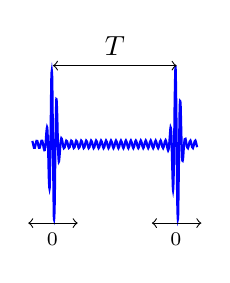
\begin{tikzpicture}
		\def\left{-1*pi/4}
		\def\right{1*pi/4}
		\def\pattern{pi/10}
		\def\pulse{100}
		\draw [domain=-pi/3:pi/3, smooth, samples=200, blue, thick] plot
		(\x,{sin(\pulse*\x r) * (0.05 + exp(-((\x-\left)*(\x-\left)) * 3 * \pulse) +
		exp(-((\x-\right)*(\x-\right)) * 3 * \pulse)});
		\draw (\left - \pattern, -1)[<->] -- (\left + \pattern, -1);
		\draw (\left, -1) node[below] {\(\ksize_0\)};
		\draw (\right - \pattern, -1)[<->] -- (\right + \pattern, -1);
		\draw (\right, -1) node[below] {\(\ksize_0\)};
		\draw (\left, 1)[<->] -- (\right, 1);
		\draw (0, 1) node[above] {\(T\)};
	\end{tikzpicture}
	\caption{Two EM patterns separated by one clock cycle.}
	\label{fig:kernel_size}
\end{wrapfigure}
\autoref{fig:kernel_size} sketches an EM trace chunk of about one clock cycle.
We make the underlying assumption that the relevant information to extract from the traces is contained in the patterns occurring around each clock, mostly due to the change of states in the memory registers storing the sensitive variables~\cite{mangard_power_2007}.%
\footnote{This assumption has somehow already been used for the pattern extraction re-alignment in \autoref{sec:visual_inspect}.}
Moreover, no additional relevant pattern is assumed to be contained in the trace until the next clock cycle, appearing \(T=50\) samples later.%
\footnote{
	We recall that despite the effect of code polymorphism, and in absence of hardware jitter, the duration of the clock period, in terms of samples, is roughly constant.
}
By carefully setting \(\ksize_0\) to the size of the EM patterns, and \(\pstride_0\) such that \(\ksize_0 \leq \pstride_0 \leq T\), we optimally extract the relevant information from the patterns while avoiding the entanglement between two of them.
In our experiments, we arbitrarily set \(\pstride_0=25\).
This first tweaked convolutional block has then the same receptive field than one would have with two normal blocks of parameters (\(\ksize=11, \pstride=5\)).
Therefore, we spare one block (\ie{} the last one), which decreases the number of learning parameters: our architecture now represents \(84,380\) (resp. \(177,500\)) learning parameters for the model attacking the \mbedTLS{} implementation (resp. \aeshuitbit{}).
\autoref{table:cnn_archi} provides a synthesis of the description of our architecture, along with a comparison with the Kim \etal{} and Zaid \etal{}'s works.
\begin{table}[h]
	\centering
	\caption{Our architecture and the recommendations from the literature.
	In the Zaid \etal{}'s methodology, \(T\) denotes the maximum assumed amount of random shift in the traces, and \(I\) denotes the assumed number of leakage temporal points in the traces.}
	\begin{tabular}{rrrr}
		\toprule
		& Kim \etal{}~\cite{kim_make_2019} & \(\enspace \) Our archi. & \enspace Zaid \etal{}~\cite{zaid_methodology_2019} \vspace{5pt}\\
		\midrule
		\(n_1\) & 1 & 0 & 2\\
		\(n_2\) & \(\log_{\pstride}(\traceLength)\) & \(\log_{\pstride}(\traceLength)\) & 3 \vspace{5pt}\\
		\(\pstride\) & 2 & \(5 (\pstride_0 = 25)\) & \(2, \frac{T}{2}, \frac{\traceLength}{I}\) \vspace{5pt}\\
		\(\ksize\) & 3 & \(11 (\ksize_0 = 10)\) & \(1, \frac{T}{2}, \frac{\traceLength}{I}\) \vspace{5pt}\\
		\(\numFilters_n\) & \(\min(\numFilters_0\times2^n, \numFilters_{\max})\) & \(10, \enspace 20, \enspace 40, \enspace 40, \enspace 80, \enspace 100 (100)\) & \(\numFilters_0\times2^n\) \vspace{5pt}\\
		\(\numFilters_0\) & 8 & 10 & \(8, \enspace 32\) \vspace{5pt}\\
		\(\numFilters_{\max}\) & 256 & 100 & - \vspace{5pt}\\
		\bottomrule
	\end{tabular}
	\label{table:cnn_archi}
\end{table}

\paragraph{Training Settings}
The source code is implemented in \textsf{Python} with the same machine as presented in \autoref{sec:implementing_dnns}.
For each experiment, the whole dataset is split into a training and a test subsets, containing respectively \(95,000\) and \(5,000\) traces.
The latter ones are used to simulate a key recovery based on the scores attributed to each hypothetical value of the sensitive target variable by the trained model.
Moreover, the \(\mathsf{SH}_{100}\) data augmentation method is applied to the
training traces, following the description given in~\cite{cagli_convolutional_2017}:
each trace is randomly shifted of maximum \(100\) points, which represents the length of \(2\) clock cycles.%
\footnote{
	This data augmentation is not applied on the attack traces.
}

The training is done by minimizing the \gls{nll} loss, with the \gls{adam} optimizer -- see \autoref{sec:optim_algo} -- during \(200\) epochs%
\footnote{
	One epoch corresponds to the number of steps necessary to pass the whole training data-set through the optimization algorithm once.
}
which approximately represents a \(16\)-hour long training for each targeted byte.
The learning rate of the optimizer is always set to \(10^{-5}\).

Based on a -- eventually partially -- trained model, we compute the efficiency of the attack, as defined by \autoref{eq:eff_sr}.